\documentclass{beamer}
\usetheme{Copenhagen}

\usepackage{siunitx}
\newcommand{\h}{\unit{\hour}}
\newcommand{\ph}{\unit{\per\hour}}
\newcommand{\um}{\unit{\micro\metre}}
\newcommand{\pums}{\unit{\per\micro\metre\squared}}
\newcommand{\nm}{\unit{\nano\mole\per\litre}}

\usepackage{amsmath}
\usepackage{amssymb}
\usepackage{cancel}
\usepackage{graphicx}
\graphicspath{ {./img/} }

\title{An ODE Model of CLASP Mutants in \emph{A. Thaliana}}
\author{Riley Wheadon}
\institute{University of British Columbia}
\date{Cytrynbaum Lab Meeting, October 2024}

\begin{document}

\frame{\titlepage}

\begin{frame}
\frametitle{Root Zonation}
\begin{figure}
    \centering
    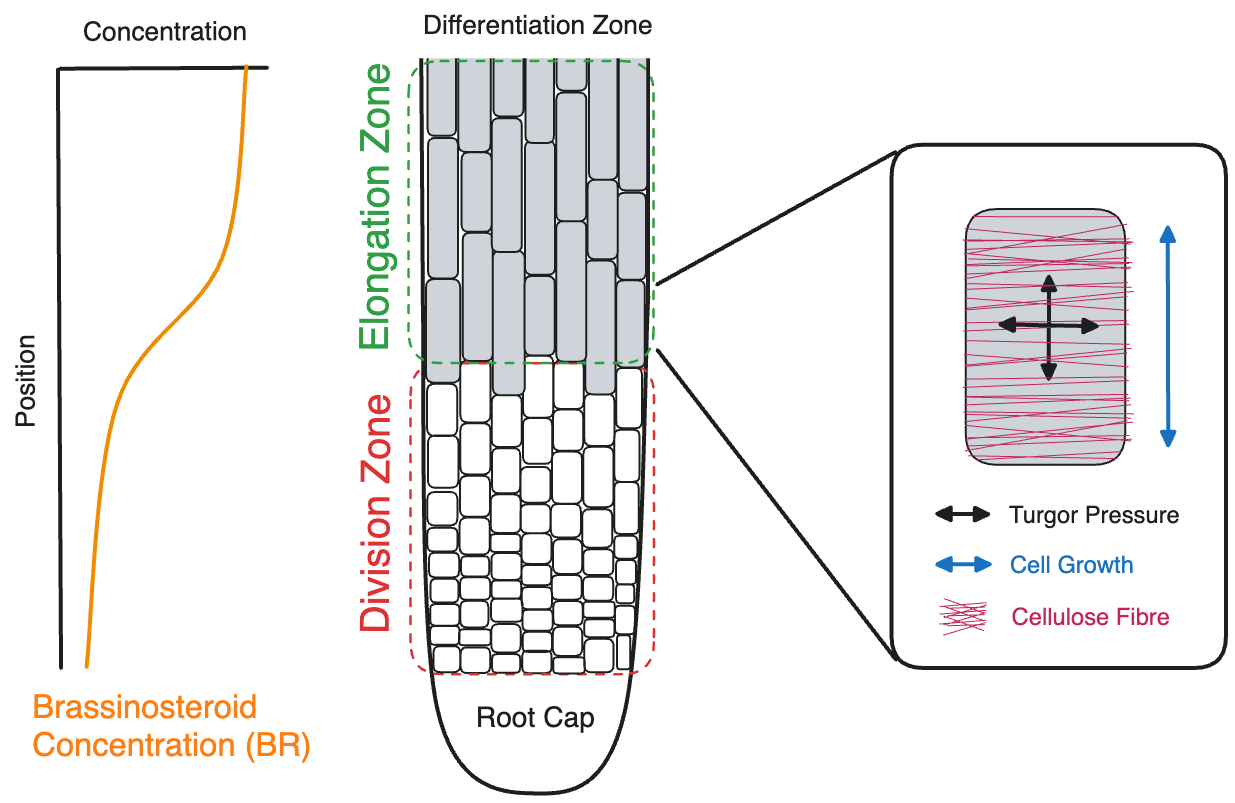
\includegraphics[height=6cm]{root-zonation.png}
    \caption{Zonation in the \emph{A. Thaliana} root. Cells growth is driven by BR. Growth is proportional to length due to the stretching of cellulose fibres.}
\end{figure}
\end{frame}

\begin{frame}
\frametitle{CLASP and Microtubules}
\begin{figure}
    \centering
    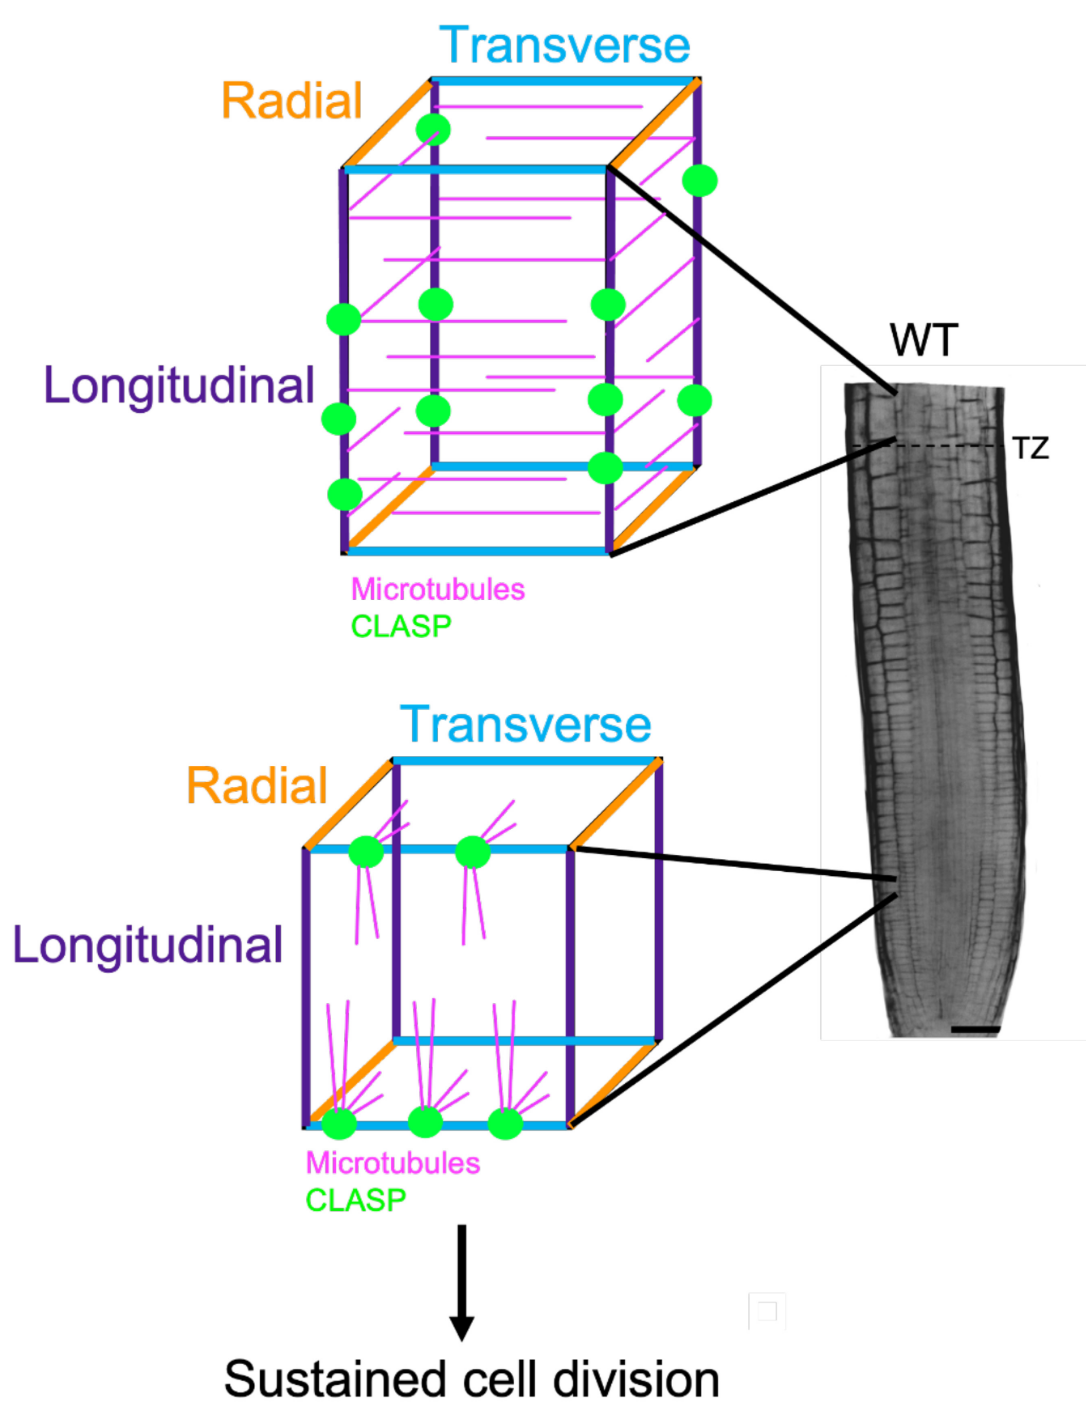
\includegraphics[height=6cm]{clasp-length-effect.png}
    \caption{Halat et al. (2022). The key takeaway from this slide is that \emph{CLASP inhibits growth, especially in shorter cells}.}
\end{figure}
\end{frame}

\begin{frame}
\frametitle{Brassinosteroid}

\begin{figure}
    \centering
    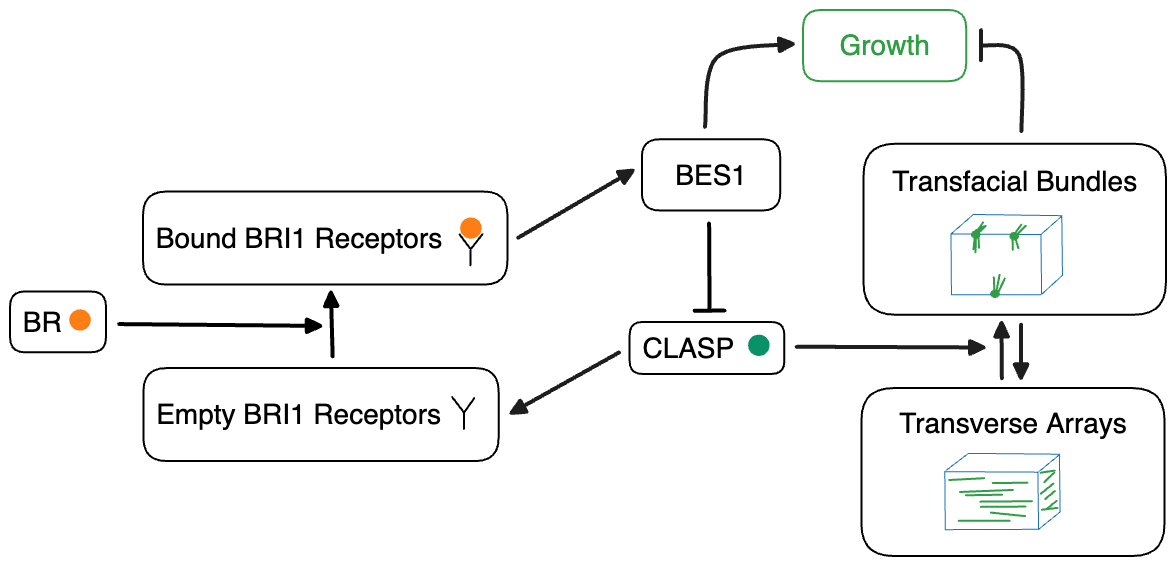
\includegraphics[width=10cm]{br-signalling.png}
    \caption{A simplified sketch of the brassinosteroid signalling network.}
\end{figure}
\end{frame}

\begin{frame}
\frametitle{Mutant Roots}
\begin{figure}
    \centering
    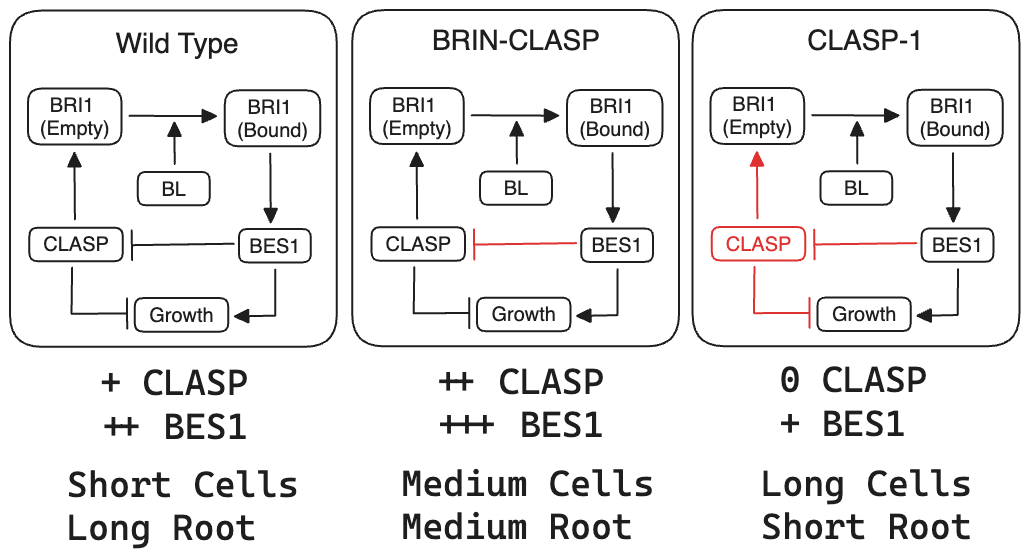
\includegraphics[width=10cm]{mutant-diagram.png}
    \caption{Signalling networks in the wild type and mutants.}
\end{figure}
\end{frame}

\begin{frame}
\frametitle{Mutant Roots}
\begin{figure}
    \centering
    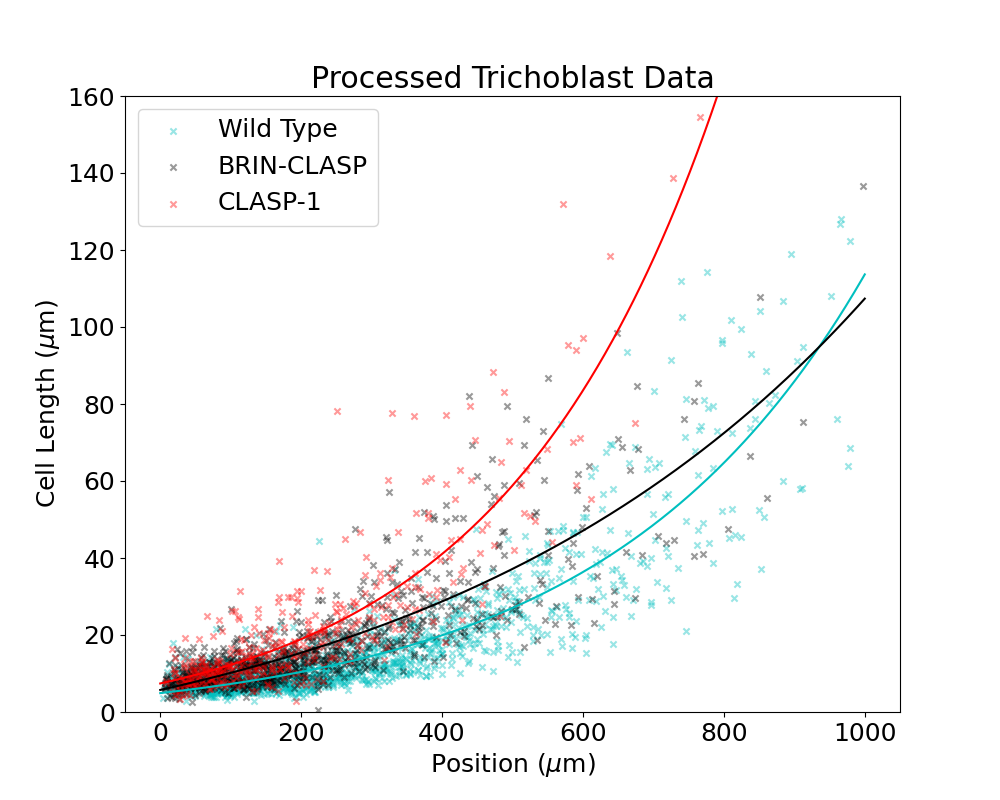
\includegraphics[height=6cm]{data-trichoblast.png}
    \caption{Experimental data from the wild type and mutants.}
\end{figure}
\end{frame}

\begin{frame}
\frametitle{Hypothesis}

\begin{figure}
    \centering
    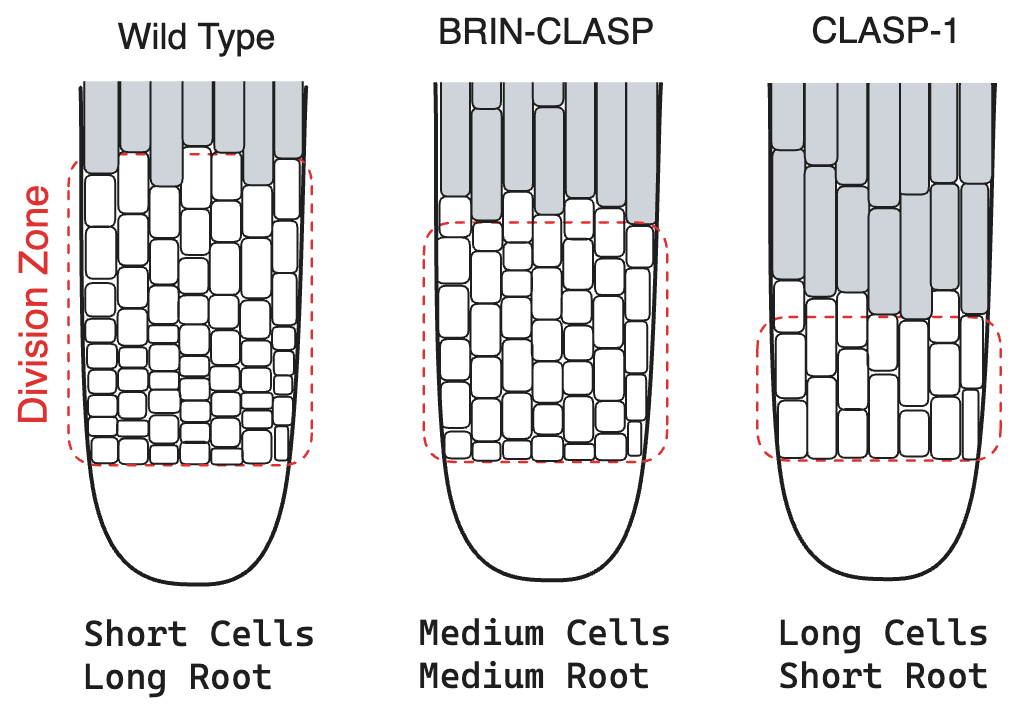
\includegraphics[height=6cm]{mutant-phenotypes.png}
    \caption{A length-driven division mechanism (might) produce the different phenotypes in the wild type, BRIN-CLASP, and CLASP-1 roots!}
\end{figure}
\end{frame}

\begin{frame}
\frametitle{Growth Model}
\begin{itemize}
    \setlength\itemsep{0.8em}
    \item We model a \emph{single column} of cells over time.
    \item Our data has no time dependence so $\Delta t$ is arbitrary.
    \item Cells grow at a basal rate $g_{0}L$. 
    \item This basal rate is inhibited by CLASP due to TFB formation.
    \item Cell growth is increased by BES1 at a rate $g_{1}PL$. We assume that BES1 signalling is linear with cell position (it is, usually).
    \item The parameter $g_{1}$ is proportional the number of receptors $R$.
\end{itemize}
\end{frame}

\begin{frame}
\frametitle{Division Model}
\begin{itemize}
    \setlength\itemsep{0.8em}
    \item Cells complete a cell cycle and divide when $D=1$.
    \item Cells also must be at least $9\um$ long to divide.
    \item Cell division creates two cells with length $L / 2$ and $D = 0$.
    \item Progress in the cell cyle proceeds at a basal rate $d_{0}$.
    \item Progress in the cell cyle is inhibited by \emph{length}. 
\end{itemize}
\medskip
\end{frame}


\begin{frame}
\frametitle{Model Equations}
In the equations below, $\text{C1}$, $\text{BC}$, and $\text{WT}$ stand in for the  CLASP-1, BRIN-CLASP, and wild type roots respectively.
$$
\begin{aligned}
    \text{C1: }\frac{ dL }{ dt } &= \left( (g_{0} - 0) + R_{\text{C1}}P  \right)L, \quad &\frac{ dD }{ dt } = d_{0}\left(1 - \frac{ L^{ n } }{ d_{L}^{ n } + L^{ n } }\right) \\[5pt]
    \text{BC: }\frac{ dL }{ dt } &= \left( (g_{0} - C_{\text{BC}}) +  R_{\text{BC}}P \right)L, \quad &\frac{ dD }{ dt } = d_{0}\left(1 - \frac{ L^{ n } }{ d_{L}^{ n } + L^{ n } }\right) \\[5pt]
    \text{WT: }\frac{ dL }{ dt } &= \left((g_{0} - C_{\text{WT}}) + R_{\text{WT}}P\right)L, \quad &\frac{ dD }{ dt } = d_{0}\left(1 - \frac{ L^{ n } }{ d_{L}^{ n } + L^{ n } }\right)
\end{aligned}
$$
Recall that $0 < C_{\text{WT}} < C_{\text{BC}}$ and $R_{\text{C1}} < R_{\text{WT}} < R_{\text{BC}}$.
\end{frame}

\begin{frame}
    \frametitle{Results (1)}
    \begin{figure}
        \centering
        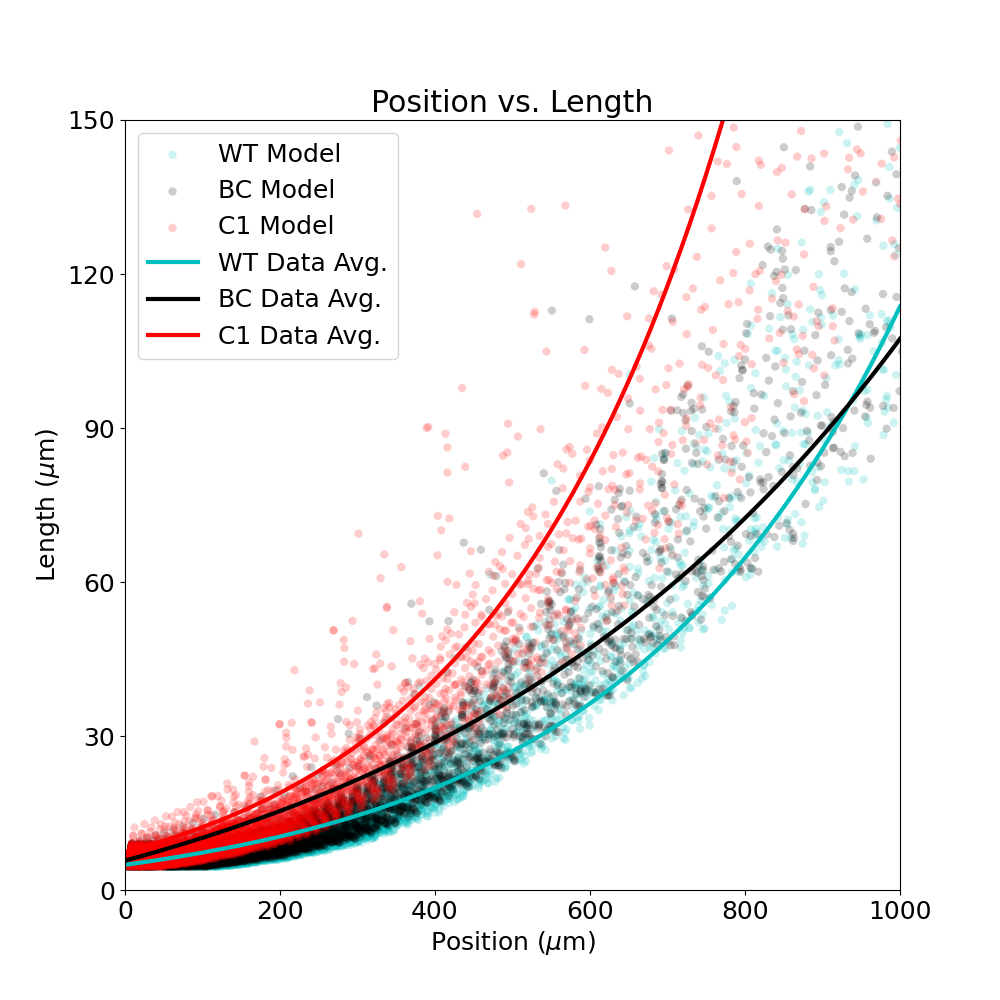
\includegraphics[height=6cm]{column-position-length.png}
        \caption{Fitted cell column model compared to data.}
    \end{figure}
\end{frame}

\begin{frame}
\frametitle{Results (2)}
\begin{table}
\begin{center}
    \begin{tabular}{ |c|c|c| }
    \hline
     Parameter & Units & Value \\
     \hline
     $g_{0}$ & $1/t$ & $0.02500$ \\ 
     $c_{\text{WT}}$ & $1/t$ & $0.01400$ \\ 
     $c_{\text{BC}}$ & $1/t$ & $0.02200$ \\ 
     $R_{\text{C1}}$ & $1/(\um \cdot t)$ & $0.00028$ \\ 
     $R_{\text{WT}}$ & $1/(\um \cdot t)$ & $0.00029$ \\ 
     $R_{\text{BC}}$ & $1/(\um \cdot t)$ & $0.00030$ \\ 
     $d_{0}$ & $D/t$ & $0.05000$ \\ 
     $d_{L}$ & $\um$ & $20.0000$ \\ 
     $n$ & $1$ & $20.0000$ \\ 
     \hline
    \end{tabular}
\caption{Parameter values for cell column model.}
\end{center}
\end{table}


\end{frame}

\begin{frame}
    \frametitle{Results (3)}
    \begin{figure}
        \centering
        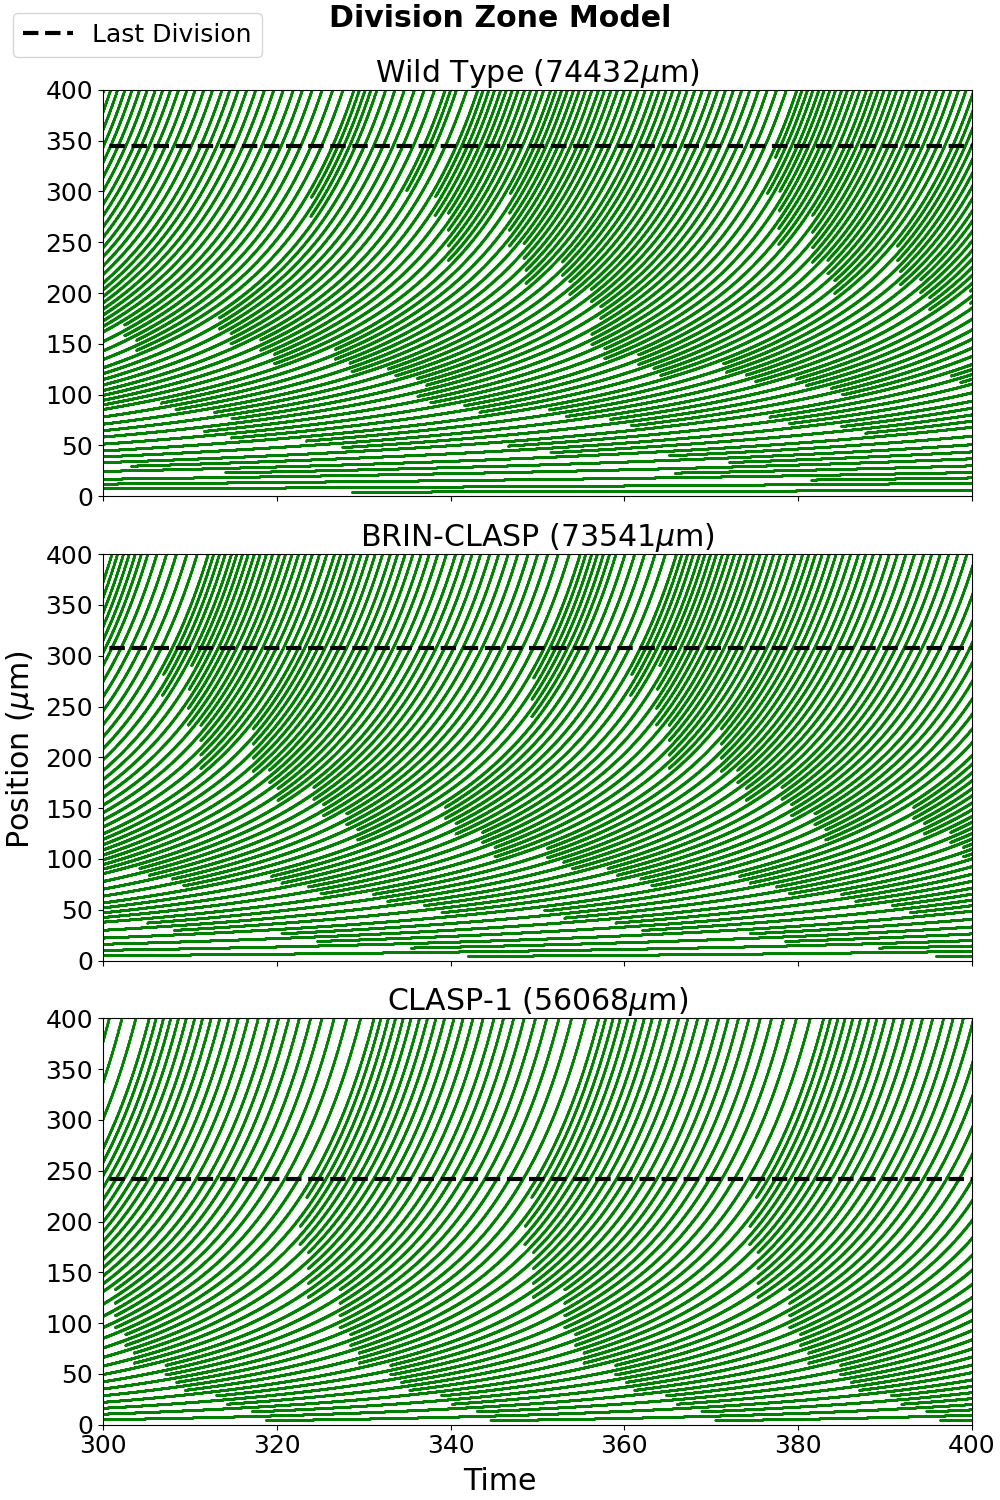
\includegraphics[height=6cm]{column-division-zone.png}
        \caption{Division zone behaviour in $t = [300, 400]$.}
    \end{figure}
\end{frame}

\begin{frame}
\frametitle{Results (4)}
\begin{figure}
    \centering
    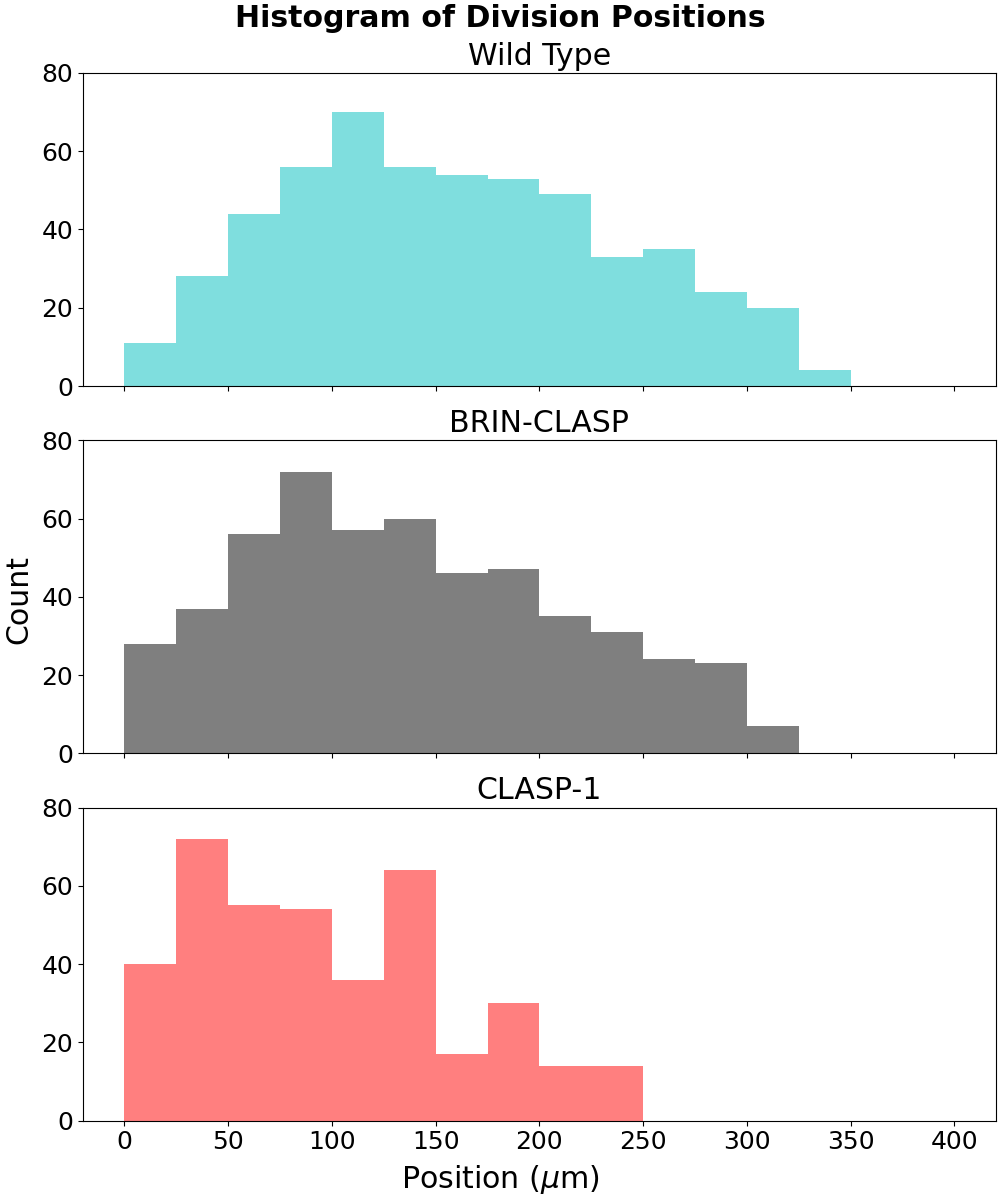
\includegraphics[height=6cm]{column-division-histogram.png}
    \caption{Division positions by mutant for the entire simulation.}
\end{figure}
\end{frame}

\begin{frame}
\frametitle{Results (5)}
\begin{table}
    \begin{center}
        \begin{tabular}{ |c|c|c|c|c| } 
        \hline
        Model & Mean Div. & Median Div. & Max Div. & \# Divs.  \\
        \hline
        Wild Type & $158.51$ & $151.41$ & $344.34$ & $537$  \\
        BRIN-CLASP & $138.26$ & $131.49$ & $307.45$ & $523$  \\
        CLASP-1 & $96.28$ & $83.80$ & $241.98$ & $396$  \\
        \hline
        \end{tabular}
    \caption{Overview of division behaviour in cell column models.}
    \end{center}
\end{table}
\end{frame}

\begin{frame}
\frametitle{Results (6)}
\begin{figure}
    \centering
    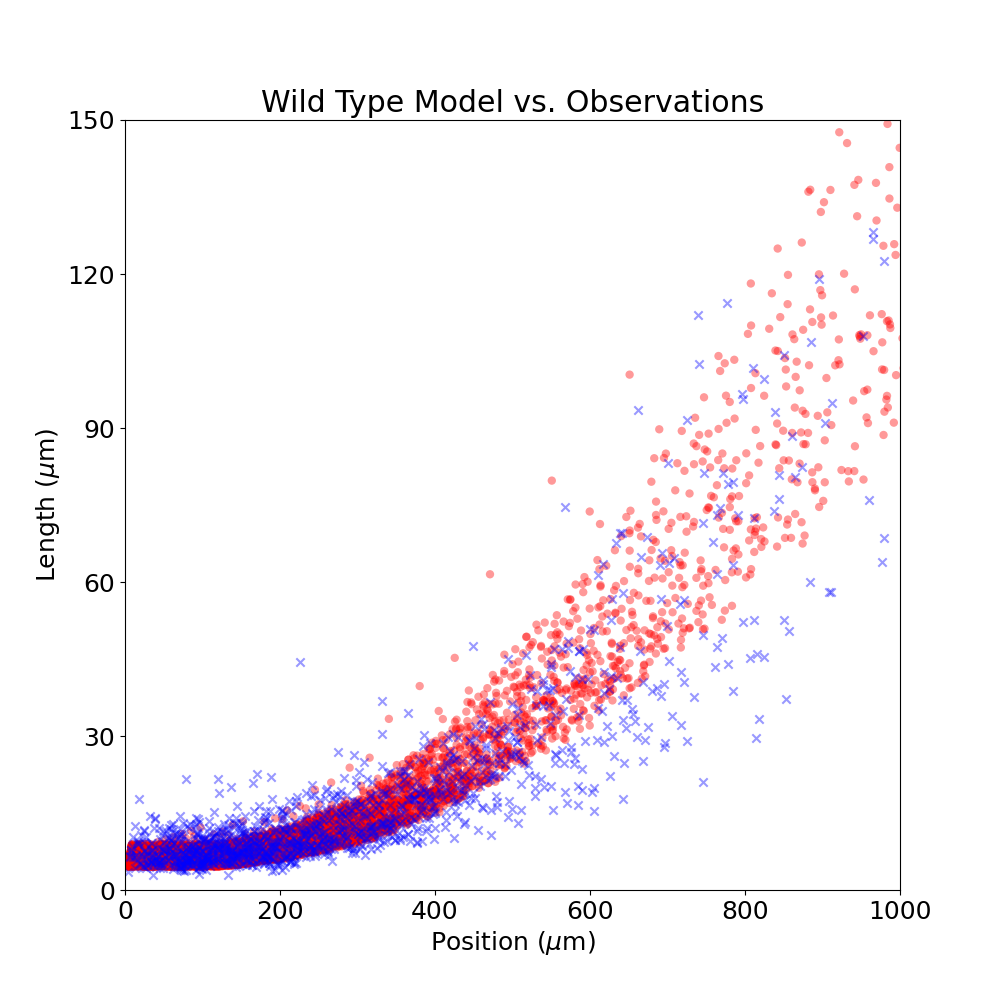
\includegraphics[height=6cm]{column-wild-type.png}
    \caption{Comparison of wild type model to observations.}
\end{figure}
\end{frame}
\begin{frame}
\frametitle{Results (7)}
\begin{figure}
    \centering
    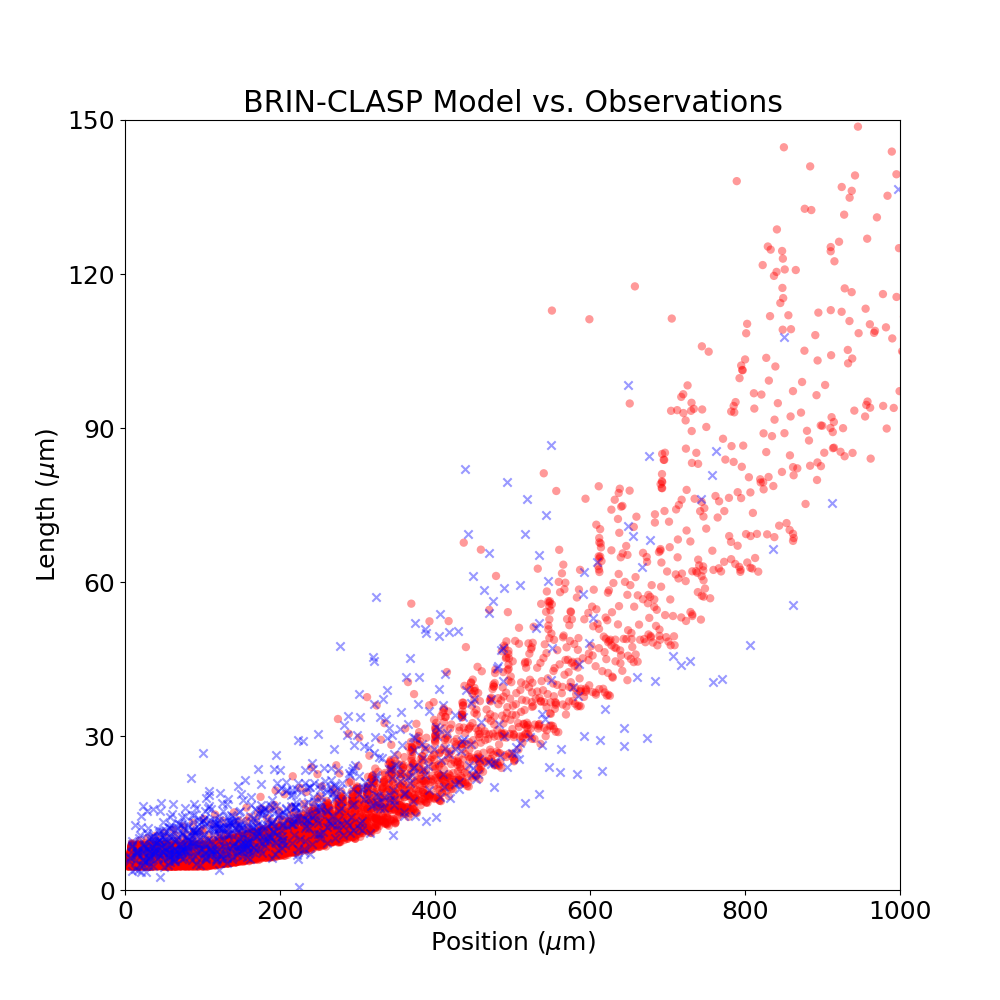
\includegraphics[height=6cm]{column-brin-clasp.png}
    \caption{Comparison of BRIN-CLASP model to observations.}
\end{figure}
\end{frame}
\begin{frame}
\frametitle{Results (8)}
\begin{figure}
    \centering
    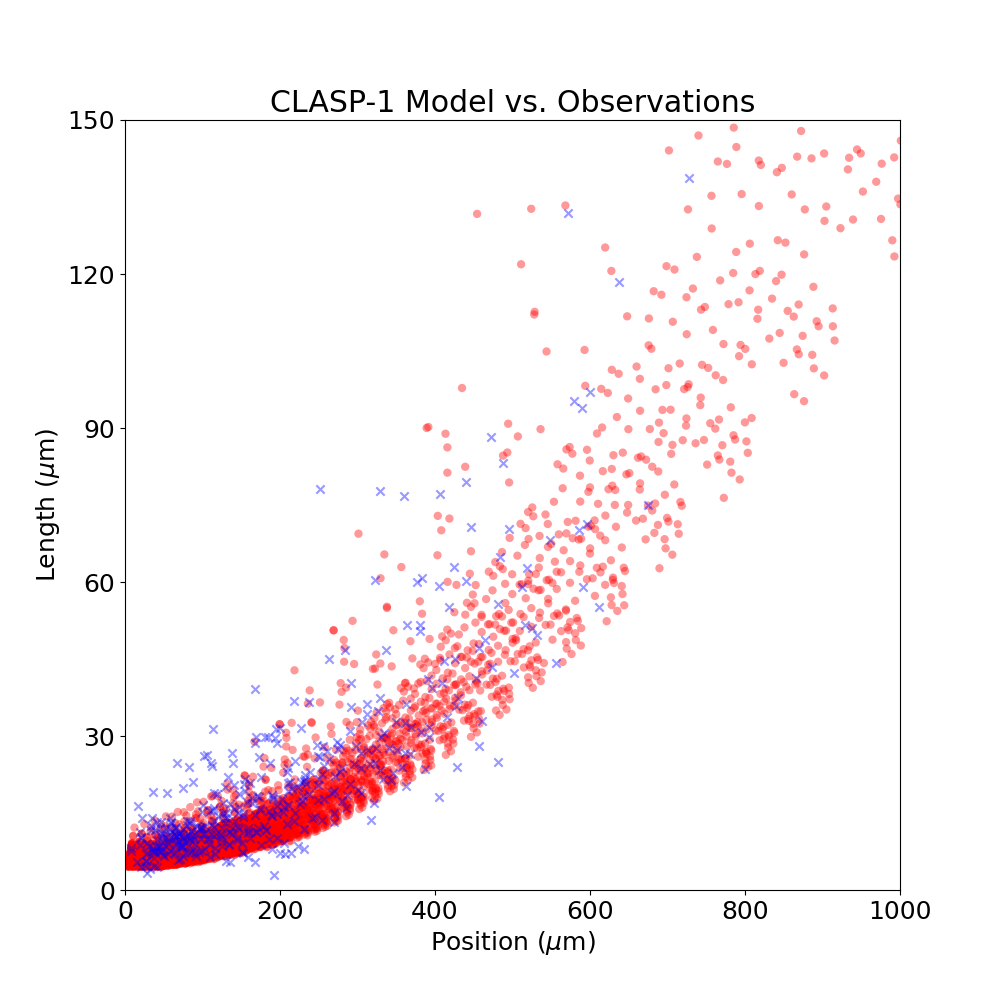
\includegraphics[height=6cm]{column-clasp-1.png}
    \caption{Comparison of CLASP-1 model to observations.}
\end{figure}
\end{frame}


\end{document}


